\section{Driving Algorithm Concept}

\subsection{Overview}
The approach of the new driving algorithm is as follows. At first, the ghostcar drives a non-competitive initial round where it takes the measurement of the
track with an optical sensor and then calculates the maximum velocity for each measured position of the track. This mapping of the track consists of pairs
$(pos_{n}, v_{max}[pos_{n}]))$ which map a track position $pos_{n}$ to an associated maximum allowed velocity at this position $v_{max}[pos_{n}]$ as demonstrated in
figure \ref{fig:PositionVelocityMapping}.
 
\begin{figure}[h]
\centering
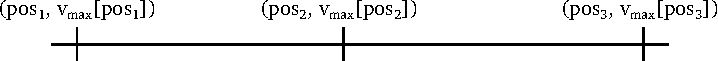
\includegraphics[width=\columnwidth]{position_velocity_mapping}
\caption{Mapping of the particular maximum allowed velocities to the corresponding recorded positions of the track.}
\label{fig:PositionVelocityMapping}
\end{figure}

The track mapping is then used to control the actual velocity of the ghostcar. For a rather optimal driving behavior and speed, it is essential to
brake early enough and not only when the car starts to slip because then it is already too late. To brake early enough, one has to look ahead in the track mapping and adapt
the current velocity appropriate to the following track sections. Now the question is how far has to be look ahead. To stay in either case on the track,
it must be possible to brake timely from the current velocity to the smallest maximum velocity. The smallest maximum velocity is the lowest velocity of all
maximum velocities and thus the lowest velocity that is needed on a certain point of the track to stay on the track.


\subsection{Calculation of the Maximum Velocity}

As already mentioned, the track mapping consists of pairs $(pos_{n}, v_{max}[pos_{n}]))$ which map a track position $pos_{n}$ to an associated maximum allowed
velocity at this position $v_{max}[pos_{n}]$. The maximum allowed velocity at a certain position is the maximum velocity at which the car stays barely on the
track. To get thrown out of the track, the car has to tilt so far that the bolt of the car is out of the track. Therefore, the maximum allowed velocity is
exactly the velocity at which the car just doesn't start to tilt. This whole situation is shown in figure \ref{fig:CarChassis}.

\begin{figure}[h]
\centering
\includegraphics[width=\columnwidth]{car_chassis}
\caption{Forces and torques that act on the ghostcar while driving a right hand bend.}
\label{fig:CarChassis}
\end{figure}

The maximum allowed velocity $v_{max}[pos_{n}]$ for a certian position $pos_{n}$ can be calculated by the following equations:

\begin{flalign}
\sum M &= M_{gm} - M_{c} = 0 \label{eq:straightx}\\
&= (F_{g} + F_{m}) \cdot l_{s} - F_{c} \cdot h_{s} \\
F_{c} \cdot h_{s} &= (F_{g} + F_{m}) \cdot l_{s} \\
\frac{m}{r} \cdot v_{max}^{2} \cdot h_{s} &= (m \cdot g + F_{m}) \cdot l_{s} \\
v_{max}^{2} &= \frac{(m \cdot g + F_{m}) \cdot l_{s}}{\frac{m}{r} \cdot h_{s}} \\
v_{max} &= \sqrt{\frac{(m \cdot g + F_{m}) \cdot l_{s}}{m \cdot h_{s}} \cdot r} \\
v_{max} &= K_{car} \cdot \sqrt{r}, \qquad K_{car} = \sqrt{\frac{(m \cdot g + F_{m}) \cdot l_{s}}{m \cdot h_{s}}}
\end{flalign}

In order to stay on the track and not to tilt, the torque against ground $M_{gm}$ has to be greater as or at least equal to the overturning torque $M_{c}$. The
force that leads to the torque against ground is the sum of the weight force $F_{g} = m \cdot g$ and the magnetic force $F_{m}$. On the other side, the force
which is responsible for the overturning torque is the centrifugal force $F_{c} = \frac{m}{r} \cdot v^{2}$ \cite{wikipedia:CentrifugalForce}. After inserting
and transposing the equations appropriately, one gets a function for the maximum allowed velocity $v_{max}$. This function can now be used to compute the maximum allowed velocity for each
recorded position of the track. As one can see in the equations above, the maximum allowed velocity depends on a constant factor $K_{car}$ and the square root
of the radius $r$ of the particular curve. The constant factor $K_{car}$ can be determined by trial and error. The radius of the particular curves can be
calculated by $r = \frac{v}{\omega}$, where $v$ is the actual velocity of the ghostcar and $\omega$ is the angular velocity of the ghostcar measured by the
gyro sensor of the car.

Now that we have the track mapping with the recorded positions and the maximum allowed velocity to each position, we can calculate the needed
look-ahead-distance.


\subsection{Calculation of the look-ahead-distance}

To calculate the needed look-ahead-distance, one has to calculate the distance that is needed by the car to be able to timely brake from the current velocity
to the smallest maximum velocity. So, the ghostcar has to be able to timely brake from the current position to the position with the smallest maximum velocity.
This means, the distance between the current position and the position with the smallest maximum velocity has to be big enough to be able to brake in this
distance from the current velocity down to the smallest maximum velocity. This situation is visualized in figure \ref{fig:TrackSections}. Therefore, one has to
know the acceleration with which the ghostcar brakes. Since the ghostcar uses an electric motor, the acceleration is actually not constant and has to be
evaluated by trial and error.

\begin{figure}[h]
\centering
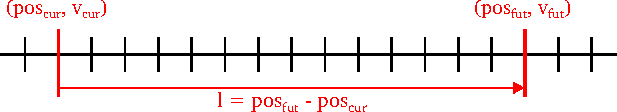
\includegraphics[width=\columnwidth]{track_sections}
\caption{Visualization of the look-ahead-distance $l$.}
\label{fig:TrackSections}
\end{figure}

Since the measured positions during driving aren't every time exacty the positions which were recorded in the initial round, this actual measured positions have
to be mapped to a recorded $(pos_{n}, v_{max}[pos_{n}]))$ pair. This is demonstrated in figure \ref{fig:CurrentPositionMapping} and
\ref{fig:FuturePositionMapping}.

\begin{figure}[h]
\centering
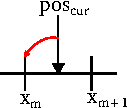
\includegraphics[width=0.25\columnwidth]{current_position_mapping}
\caption{Mapping of the current position to a recorded $(pos_{n}, v_{max}[pos_{n}]))$ pair.}
\label{fig:CurrentPositionMapping}
\end{figure}

\begin{figure}[h]
\centering
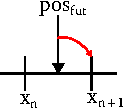
\includegraphics[width=0.25\columnwidth]{future_position_mapping}
\caption{Mapping of the future position to a recorded $(pos_{n}, v_{max}[pos_{n}]))$ pair.}
\label{fig:FuturePositionMapping}
\end{figure}

Now we have to determine the equations for calculation of the needed look-ahead-distance. Therefore, we have to evaluate the distance that is needed to brake
from the current velocity to the target velocity \cite{TimeAndDistanceCalculationFromAcceleration}. To do so, at first the time $t$ needed to brake from the
initial velocity $v_{i}$ to the final velocity $v_{f}$ with a certain acceleration $a$ has to be calculated:

\begin{flalign}
v_{f} - v_{i} = a \cdot t \\
t = \frac{v_{f} - v_{i}}{a} \\
t = \frac{v_{min} - v_{cur}}{a} \\
\end{flalign}

Knowing the time $t$ needed to brake from the current velocity $v_{cur}$ down to the smallest maximum velocity $v_{min}$, one can compute the distance $l$ which
the car drives in this time while braking with a certain constant acceleration $a$. This distance $l$ is the needed look-ahead-distance.

\begin{flalign}
l = v_{i} \cdot t + \frac{a \cdot t^{2}}{2} \\
l = v_{cur} \cdot t + \frac{a \cdot t^{2}}{2} \\
l = v_{cur} \cdot \frac{v_{min} - v_{cur}}{a} + \frac{a \cdot (\frac{v_{min} - v_{cur}}{a})^{2}}{2} \\
l = v_{cur} \cdot \frac{v_{min} - v_{cur}}{a} + \frac{(v_{min} - v_{cur})^2}{2a} \\
\end{flalign}

As one can see, the needed look-ahead-distance $l$ depends on the current velocity $v_{cur}$ (determined by the position changes and the time needed for that
changes), the smallest maximum velocity $v_{min}$ (smallest velocity of all calculated maximum velocities) and the braking acceleration $a$ (evaluated by trial
and error).
